% $HeadURL$

\paragraph{Macromolecule}
\label{sec:macromolecule}

Many biological processes involve \emph{macromolecules}: biochemical substances that are built up from the covalent linking of pseudo-identical units.  Examples of macromolecules include proteins, nucleic acids (RNA, DNA), and polysaccharides (glycogen, cellulose, starch, etc.).  Attempting to define a separate glyph for all of these different molecules would lead to an explosion of symbols in SBGN, so instead, \SBGNPDLone defines only one glyph for all macromolecules.  The same glyph is to be used for a protein, a nucleic acid, a complex sugar, and so on.  The exact nature of a particular macromolecule in a map is then clarified using its label and decorations, as will become clear below.  (Future levels of SBGN may subclass the \glyph{macromolecule} and introduce different glyphs to differentiate between types of macromolecules.)

\begin{glyphDescription}
\item[Identifying Attributes:]\mbox{}
  \begin{itemize}
  \item owning compartment
  \item name
  \item cardinality
  \item The set of state values associated with this EPN.
 \end{itemize}
\item[Special constraints or rules:]\mbox{}\newline The mutimer glyph
  must be used if cardinality is greater than 1.
\end{glyphDescription}

\subparagraph{Glyph: \glyph{Macromolecule monomer}}

This glyph represents a monomeric macromolecule.

\begin{glyphDescription}

\glyphSboTerm SBO:0000245 ! macromolecule 

\glyphContainer A macromolecule is represented by a rectangular container with rounded corners, as illustrated in \fig{macromolecule}.

\glyphLabel A \glyph{macromolecule} is identified by a label placed in an unbordered box containing a string of characters.  The characters can be distributed on several lines to improve readability, although this is not mandatory.  The label box must be attached to the center of the container.  The label may spill outside of the container.

\glyphAux A \glyph{macromolecule} can carry state variables that can add information about its state (\sect{stateVariable}).  The state of a macromolecule is therefore defined as the set of all its state variables. 

A \glyph{macromolecule} can also carry one or several \glyph{units of information} (\sect{unitInfo}).  The units of information can characterize a domain, such as a binding site.  Particular \glyph{units of information} are available for describing the material type (\sect{material-types-cv}) and the conceptual type (\sect{conceptual-types-cv}) of a macromolecule.  

\glyphCloning Labeled Clone Marker.

\end{glyphDescription}

\begin{figure}[H]
  \centering
  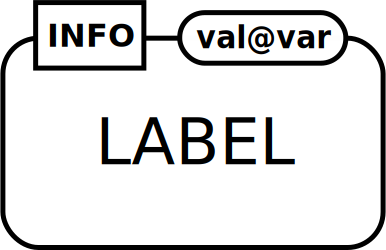
\includegraphics[width = 3in]{images/macromolecule}
  \caption{The \PD glyph for \glyph{macromolecule}, shown plain and
    unadorned on the left, and with with an additional state variable and a
    unit of information in the right and the cloned form on the right.}
  \label{fig:macromolecule}
\end{figure}


\subparagraph{Glyph: \glyph{Macromolecule multimer}}

This glyph represents a multimeric macromolecule.

\begin{glyphDescription}

\glyphSboTerm SBO:0000420 ! multimer of macromolecules

A \glyph{multimer} is represented by two identical containers shifted horizontally and vertically and stacked one on top of the other.  \fig{macromolMultimer} illustrates the glyph.

\glyphLabel As monomer

\glyphAux As monomer.

\glyphCloning Labeled Clone Marker.

\end{glyphDescription}

\begin{figure}[H]
  \centering
  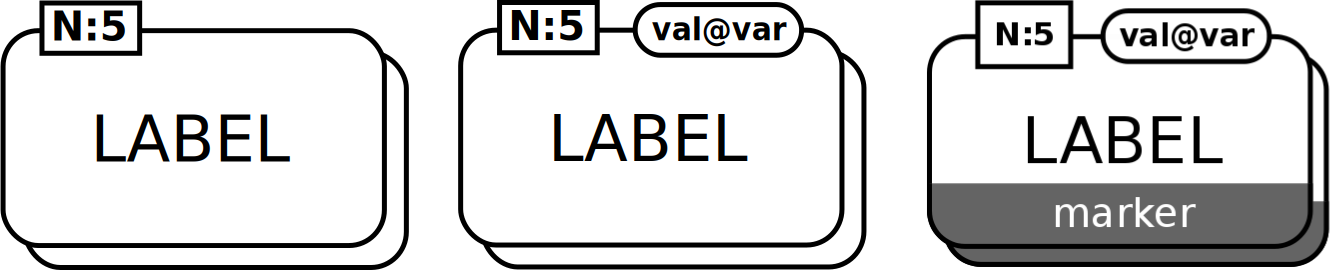
\includegraphics[width = 3.0in]{images/macromolMultimer}
  \caption{The \PD glyph for \glyph{macromolecule multimer}, shown plain and
    unadorned on the left, and with with an additional state variable and a
    unit of information on the right.}
  \label{fig:macromolMultimer}
\end{figure}




% The following is for [X]Emacs users.   Please leave in place.
% Local Variables:
% TeX-master: "../sbgn_PD-level1"
% End:
